%%%%%%%%%%%%%%%%%%%%%%%%%%%%%%%%%%%%%%%%%

\chapter{Ultracold neutrons}\label{chap:UCN}

%%%%%%%%%%%%%%%%%%%%%%%%%%%%%%%%%%%%%%%%%

Ultracold neutron(s) (\ucn) are neutrons of very low kinetic energy ($\lesssim$\qty{300}{\nano\eV}) and have a number of very convenient properties that make them useful in experiments involving fundamental physics. Modern nEDM experiments are performed almost exclusively using UCN \cite{BAK06, SER15, ABE20} (an alternative is proposed in Ref.~\cite{PIE13}). Depending on the optical potential, \ucn may be contained at all angles of incidence by material bottles (Sec.~\ref{sec:ucn_matter_int}). They are also of low enough energies that they may be influenced by gravitational and magnetic potentials (Sec.~\ref{sec:ucn_grav_em}). Due to the ease of manipulation and transport, \ucn can be moved away from the production source, where backgrounds are typically high, into shielded environments where backgrounds may be controlled. \ucn are easy to polarize, and their polarization is easily measured (Sec.~\ref{sec:ucn_polarizers}). Neutrons are also abundantly available (albeit bound in nuclei) and when freed have a long lifetime (Sec.~\ref{sec:weak_interaction}).

%%%%%%%%%%%%%%%%%%%%%%%%%%%%%%%%%%%%%%%%%

\section{UCN properties}

%%%%%%%%%%%%%%%%%%%%%%%%%%%%%%%%%%%%%%%%%

A population of \ucn may be treated as an ideal gas with a few unique characteristics: \cite{golubUCN}
%
\begin{itemize}
    \item \ucn wall collisions are mostly elastic and specular. Inelastic scattering results in a neutron being upscattered (heated) from the \ucn energy range and lost. \ucn gas in a container is a pseudo equilibrium where the gas velocity space is isotropic in the storage volume
    \item UCN\textendash UCN collisions are negligible, and the mean free path of a \ucn is characterized by the geometry of the storage volume
    \item Due to gravity, \ucn density tends to decrease as height increases within the storage volume.
    \item \ucn gas density decreases over time as \ucn are lost to $\beta$ decay and wall collisions.
\end{itemize}
%
\ucn flow in guide tubes is similar to rarified gas flow in tubes, with the same caveats described above.

%%%%%%%%%%%%%%%%%%%%%%%%%%%%%%%%%%%%%%%%%

\section{Gravitational and electromagnetic interactions}\label{sec:ucn_grav_em}

%%%%%%%%%%%%%%%%%%%%%%%%%%%%%%%%%%%%%%%%%

\ucn are of sufficiently low energy such that the influence of gravity is non-negligible. For gravitational acceleration $g_0$ acting on a neutron mass \gls{m_n}, the potential energy of at a height $h$ is given by
%
\begin{gather}
    V_g = \gls{mg}h
\end{gather}
%
where $\gls*{mg}=$\glsvalue*{mg} \cite{codata_2018}.

The magnetic moment of the neutron also interacts with a magnetic field \gls*{bField}, with the potential energy defined by
%
\begin{gather}
    V_m = - \vv{\gls{mu_n}}\cdot \gls*{bField}
\end{gather}
%
where $\gls*{mu_n}=60.307\,739(15)\text{ neV T}^{-1}$ \cite{codata_2018}. Spin dependent interactions in a magnetic field are further described in Chap.~\ref{chap:spinManipulation}.

The neutron charge limit is effectively zero \cite{baumann_neutron_charge}
%
\begin{gather}
    \gls*{q_n}=\glsvalue*{q_n}\quad(68 \% \text{ c.l.})
\end{gather}
%
Due to the internal charge distribution of the neutron quark structure, a neutron subjected to an external electric field creates an induced EDM given by $d_\text{induced}=4\pi \epsilon_0 \alpha_\text{n} E$. The neutron polarizability $\alpha_\text{n}$ is $(11.8\pm 1.1)\,10^{-4}\text{ fm}^3$ \cite{pdg2022}, giving $d_\text{induced}\sim 10^{-32}e\,\text{cm}$. This is well below the sensitivity of the \acrshort*{lanl} \acrshort*{nedm} experiment.


%%%%%%%%%%%%%%%%%%%%%%%%%%%%%%%%%%%%%%%%%

\section{Weak interaction}\label{sec:weak_interaction}

%%%%%%%%%%%%%%%%%%%%%%%%%%%%%%%%%%%%%%%%%

\begin{figure}[htp]
    \centering
    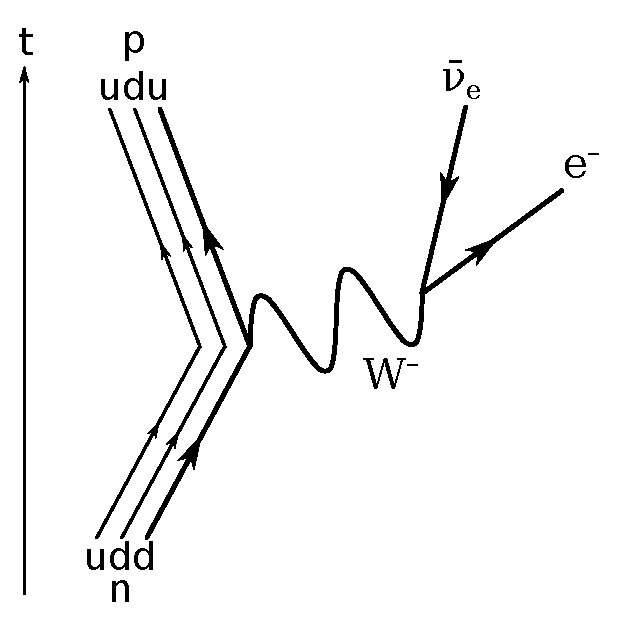
\includegraphics[width=0.3 \textwidth]{figures/beta_negative_decay.pdf}
    \caption[Feynman diagram of free neutron $\beta$ decay]
    {Feynman diagram of free neutron $\beta$ decay. Image from \cite{beta_decay_fig}}
    \label{fig:beta_decay}
\end{figure}

Free neutrons undergo $\beta$ decay
%
\begin{gather}
    n\rightarrow p+ e^-+\bar{\nu}_e
\end{gather}
%
governed by the neutron lifetime $\gls{tau_n}=\glsvalue*{tau_n}$ \cite{pdg2022}. The Feynman diagram for this process is given in Fig.~\ref{fig:beta_decay}. The neutron lifetime designates the amount of helium created during Big Bang nucleosynthesis. The CKM matrix element $V_\text{ud}$ can also be determined from measurements of \gls{tau_n} in combination with measurements of $0^+\rightarrow0^+$ decays \cite{Young2014}.

The most accurate neutron lifetime experiments to date have been storage experiments with \ucn held by magnetic and gravitational potentials, such as the UCN$\tau$ experiment at \acrshort{lanl} \cite{gonzalez_ucn_tau}. There is an ongoing disagreement between neutron lifetime storage experiments that count surviving \ucn and neutron lifetime cold beam experiments that count the proton decay products~\cite{czarnecki2018}.

The neutron beta decay directional distribution and total decay rate can be very generally written in terms of the neutron spin and lepton momenta \cite{Young2014}
%
\begin{align}
    d\Gamma(\vv{p}_e, \vv{p}_{\bar{\nu}}) &= dE_e\,d\Omega_e \,d\Omega_{\bar{\nu}} \frac{F(E_e)\,p_e E_e (E_o-E_e)^2}{(2\pi)^5} \xi \nonumber \\
    &\quad\quad \times \left[1 + a\frac{\vv{p}_e \cdot \vv{p}_{\bar{\nu}}}{E_e E_{\bar{\nu}}}
    +b\frac{m_e}{E_e} + \langle \vv{S}_\text{n} \rangle \cdot
    \left( A\frac{\vv{p}_e}{E_e} + B \frac{\vv{p}_{\bar{\nu}}}{E_e} + D\frac{\vv{p}_e\times \vv{p}_{\bar{\nu}}}{E_e E_{\bar{\nu}}}
    \right) \right]
\end{align}
%
$\vv{S}_\text{n}$ is neutron spin, $F(E_e)$ is the Fermi function for final state interactions, $E_o$ is the endpoint energy, $E_e$ and $\vv{p}_e$ are electron energy and momentum, and $E_{\bar{\nu}}$ and $\vv{p}_{\bar{\nu}}$ are anti-neutrino energy and momentum.

Of interest are correlation coefficients $a$, $b$, $A$, $B$, and $D$, which are experimental observables. Measurements of these coefficients are a probe of the V\textendash A structure of the \acrshort*{sm}. 
%
\begin{itemize}
    \item Electron-antineutrino asymmetry $a$ is measured from the proton spectrum.
    \item Fierz interference coefficient $b$ is measured from the $\beta$ spectrum. $b$ is nominally $0$ in the \acrshort*{sm}.
    \item Beta asymmetry $A$ is determined from the angular correlation between the emitted electron and neutron polarization.
    \item Spin-antineutrino asymmetry $B$ is found via the angular correlation of the recoil proton and neutron polarization.
    \item Triple product $D$ arises from the triple correlation between electron momentum, proton momentum, and neutron spin. $D$ is also nominally $0$ in the \acrshort*{sm}.
\end{itemize}

Reference~\cite{Young2014} provides a review of the $\beta$ decay experimental program at \acrshort{lanl}


%%%%%%%%%%%%%%%%%%%%%%%%%%%%%%%%%%%%%%%%%

\section{UCN interactions with matter}\label{sec:ucn_matter_int}

%%%%%%%%%%%%%%%%%%%%%%%%%%%%%%%%%%%%%%%%%

%%%%%%%%%%%%%%%%%%%%%%%%%%%%%%%%%%%%%%%%%

\subsection{Neutron transmission through material}

%%%%%%%%%%%%%%%%%%%%%%%%%%%%%%%%%%%%%%%%%

\comment{Rogel pg. 59. Schreyer thesis}

